\documentclass[brazil,ruledheader]{abntifes}
%\documentclass[brazil,twoside,ruledheader]{abntifes}
\usepackage[T1]{fontenc} 
%\usepackage[latin1]{inputenc}
\usepackage[utf8]{inputenc}
\usepackage[brazil]{babel}
\usepackage[]{algorithm2e}
\usepackage{pslatex}
\usepackage{url}
%\usepackage{fancyhdr}
\usepackage{graphicx}
\usepackage{amsmath, amsthm, amssymb}
\usepackage{exercise}
\usepackage{makeidx}
\usepackage{setspace}
\usepackage{multicol}    
\usepackage{upquote}
\usepackage{graphicx}
\usepackage{float}
\usepackage{epigraph}

%\usepackage{kurier}					% sans serif
\usepackage[charter]{mathdesign}		% serif

% Code
\usepackage{listings}
\usepackage{sourcecodepro}
\usepackage{color}
\definecolor{bluekeywords}{rgb}{0.13,0.13,1}
\definecolor{greencomments}{rgb}{0,0.5,0}
\definecolor{redstrings}{rgb}{0.9,0,0}
\renewcommand\lstlistingname{Código}
\lstset{language=C,
	frame=tb,
	showspaces=false,
	showtabs=false,
	breaklines=true,
	showstringspaces=false,
	breakatwhitespace=true,
	escapeinside={(*@}{@*)},
	commentstyle=\color{greencomments},
	keywordstyle=\color{bluekeywords},
	stringstyle=\color{redstrings},
	basicstyle=\ttfamily\footnotesize
}

% Não conta numeração de capítulos
\usepackage{chngcntr}
\counterwithout{figure}{chapter}
\AtBeginDocument{\counterwithout{lstlisting}{chapter}}

\lstdefinelanguage{glsl}
{
	morekeywords={new,struct,null,switch,
		base,extern,object,this,bool,false,operator,throw,
		break,out,true,byte,fixed,override,try,
		case,float,params,typeof,catch,for,private,uint,
		char,foreach,protected,ulong,public,
		class,if,const,implicit,ref,ushort,
		continue,in,return,using,decimal,int,sbyte,virtual,
		default,interface,sealed,short,void,do,is,sizeof,while,double,lock,else,long,static,enum,string,uniform,layout,version},
	sensitive=false,
	morecomment=[l]{//},
	morecomment=[s]{/*}{*/},
	morestring=[b]",
}
  
\lstdefinelanguage{C}
{
	morekeywords={abstract,event,new,struct,as,explicit,null,switch
	base,extern,object,this,bool,false,operator,throw,
	break,finally,out,true,byte,fixed,override,try,
	case,float,params,typeof,catch,for,private,uint,
	char,foreach,protected,ulong,checked,goto,public,unchecked,
	class,if,readonly,unsafe,const,implicit,ref,ushort,
	continue,in,return,using,decimal,int,sbyte,virtual,
	default,interface,sealed,volatile,delegate,internal,short,void,do,is,sizeof,while,double,lock,stackalloc,
	else,long,static,enum,namespace,string,uniform,layout},
	sensitive=false,
	morecomment=[l]{//},
	morecomment=[s]{/*}{*/},
	morestring=[b]",
}

\newcommand{\AUTOR}{Gabriel Sussumu Kato}
\newcommand{\SEGUNDOAUTOR}{}
\newcommand{\ORIENTADOR}{D.Sc. Sicilia Ferreira Ponce Pasini Judice}
\newcommand{\COORIENTADOR}{}
\newcommand{\TITULO}{INTEGRAÇÃO OPENGL E BULLET PHYSICS}
\newcommand{\CURSO}{Tecnólogo em Tecnologia da Informação e da Comunicação}
\newcommand{\GRAU}{Tecnólogo em Tecnologia da Informação e da Comunicação}
% \newcommand{\GRAU}{Tecnólogo em Análise e Desenvolvimento de Sistemas}
\newcommand{\INSTITUICAO}{Faculdade de Educação Tecnológica do Estado do Rio de Janeiro Faeterj/Petrópolis}
\newcommand{\ANO}{Junho, 2016}
\newcommand{\DATA}{Dia de Mês de Ano}
\newcommand{\LOCAL}{Petrópolis - RJ}
\newcommand{\epigrafe}{\vspace{1cm}{\raggedright\par\sffamily\slshape\par}}
\begin{document}

\autor{\AUTOR}
\titulo{\TITULO}
\orientador{\ORIENTADOR}
\coorientador{\COORIENTADOR}

\comentario{Trabalho de Conclusão de Curso apresentado à Coordenadoria do Curso de \CURSO\
	    da \INSTITUICAO , como requisito parcial para obtenção do título de \GRAU .}

\instituicao{\INSTITUICAO}
\curso{\CURSO}
\governo{Governo do Estado do Rio de Janeiro}
\secretaria{Secretaria de Estado de Ciência e Tecnologia}
\fundacao{Fundação de Apoio à Escola Técnica}
\cpti{Centro de Educação Profissional em Tecnologia da Informação}
\local{\LOCAL}
\data{\ANO}

\capa

\folhaderosto

% Ficha Catalográfica
%\begin{figure}
%\includegraphics[width=11cm]{FichaCatalografica.pdf}
%\end{figure}

% Folha de Aprovação
\newpage
\vfill 
\null
\begin{center}
{\Huge {\bfseries\itshape Folha de Aprovação}}\\[3cm]
\begin{espacoduplo}
Trabalho de Conclusão de Curso sob o título \textit{``\TITULO''},
defendida por \AUTOR\ e aprovada em \DATA, em \LOCAL, pela banca examinadora constituída pelos
professores: \setlength{\ABNTsignthickness}{0.4pt}
\end{espacoduplo}
\setlength{\ABNTsignthickness}{0.4pt}

% ou inserir a página assinada e escaneada aqui
%\begin{figure}
%\includegraphics[]{Fo	lhaAprovacao.pdf}
%\end{figure}

\assinatura{Prof. \ORIENTADOR\\ Orientador} 
\assinatura{Prof. Banca Interna \\ \INSTITUICAO} 
\assinatura{Prof. Banca Interna \\ \INSTITUICAO} 
%\assinatura{Prof. Banca Externa \\ Instituto do membro externo}

\end{center}


% Folha do Termo de Compromisso
\newpage

\vfill 
\null
\begin{center}
{\Huge {\bfseries\itshape Declaração de Autor}}\\[3cm]
\begin{espacoduplo}
Declaro, para fins de pesquisa acadêmica, didática e técnico-científica, que o presente Trabalho de Conclusão
de Curso pode ser parcial ou totalmente utilizado desde que se faça referência à fonte e aos autores.
\end{espacoduplo}
\setlength{\ABNTsignthickness}{0.4pt}
\assinatura{\AUTOR}
Petrópolis, em \DATA
\end{center}


%\chapter*{Dedicatória}


%\chapter*{Agradecimentos}

\vfill 
\null

%\begin{center}
%{\Huge {\bfseries\itshape Epígrafe}}\\[3cm]
%\vspace{15cm}
%\end{center}
%\begin{espacoduplo}
%\end{espacoduplo}
% Não é obrigatorio ter epigrafe
%\epigraph{"Frase de efeito"}{(Autor)}

\begin{resumo}
Este trabalho demonstra o processo de integração entre a API (\textit{Application Programming Interface}, ou Interface de Programação de Aplicativo) gráfica OpenGL e o motor de física \textit{Bullet Physics}. Nele, foi desenvolvida uma simples demonstração onde é possível observar diversos fenômenos físicos como gravidade, colisão, inércia e fricção. Tal integração foi feita visando tornar mais agradável o aprendizado de qualquer uma das tecnologias envolvidas. A aplicação foi feita utilizando a biblioteca SDL2 (\textit{Simple DirectMedia Layer}), para tratar a criação de janelas e entrada e saída de dados do usuário em múltiplas plataformas, como Windows, MacOS e Linux. Para a criação do ambiente gráfico, foi utilizada a API gráfica multiplataforma OpenGL, escrita na versão 3.3 ou superior, também conhecida como \textit{modern}, o que possibilita utilizar recursos não existentes em versões anteriores. O motor de física Bullet tem suporte a recursos comuns, como gravidade, colisão, corpos rígidos, entre outros. Todas as bibliotecas escolhidas são de código livre. A ferramenta escolhida para o desenvolvimento foi a IDE (\textit{Integrated Development Environment}, ou Ambiente de Desenvolvimento Integrado) Visual Studio Community 2015, para Windows, também gratuita, porém é possível utilizar qualquer outro compilador para obter o mesmo resultado.
\\\\\textbf{Palavras-chave:} API gráfica. Motor de física.
\end{resumo}

\begin{abstract}
This work shows the integration process between the graphical API (Application Programming Interface) OpenGL and the physics engine Bullet Physics. It was developed a simple demonstration where it can be observed some physical phenomena like gravity, collision, inertia and friction. Such integration was created in order to make more pleasant learning any of the involved technologies. The application was made using the library SDL2 (Simple Direct Media Layer), to manage windows creation and input and output user data on multiple platforms, like Windows, MacOS and Linux. For the creation of the graphical environment, it was used the multiplatform graphical API OpenGL, written in version 3.3 or superior, also referred to as modern, what makes possible to use features not available on previous versions. The physics engine Bullet has support to common features like gravity, collision, rigid bodies, among others. All chosen libraries are open source. The selected tool for development were the IDE (Integrated Development Environment) Visual Studio Community 2015, for Windows, also free, however it is possible to use any other compiler to achieve the same result.
\\\\\textbf{Key-words:} Graphical API. Physics engine.
\end{abstract}
\listoffigures

%Lista de abreviaturas

\tableofcontents{}



% --------------------------------------------------------------------
% ---------------------------- CONTEÚDO ------------------------------
% --------------------------------------------------------------------

\chapter{Introdução}
%\chapter{APIs Gráficas}
\chapter{OpenGL}
Ao longo do final do século XX, a computação gráfica ganhou grande importância na vida de pessoas comuns. Tal tecnologia se tornou presente não apenas em usos militares como SAGE (\textit{Semi-Automatic Ground Environment}), sistema que convertia dados de radares em imagens computadorizadas (MACHOVER, 1978) na década de 50, como também em filmes como Toy Story (1995), primeiro longa-metragem completamente computadorizado (GUHA, 2010).

%\begin{figure}[h]
%	\centering
%	
\includegraphics[scale=0.3]{imagens/toy-story.jpg}
%	\caption{\small Toy Story (1995), primeiro longa-metragem completamente em CG. (Fonte: Pixar, 2016)}
%	\label{fig:toy-story}
%\end{figure}

Na década de 80, boa parte do trabalho gráfico era produzido em \textit{workstations}, que utilizavam a APIs com diferentes implementações, dificultando a produção de programas multiplataforma. Em 1982, a SGI (\textit{Silicon Graphics, Inc}) começou o desenvolvimento de sua API proprietária IRIS GL, atingindo alta popularidade (MARTZ, 2006). A pressão por uma API aberta e unificada aumentou por parte dos desenvolvedores de \textit{software}, culminando em 1991 com a formulação do OpenGL ARB (\textit{Architecture Review Board}), consórcio de empresas para regulamentar o projeto, e o lançamento da versão 1.0 no ano seguinte.

Segundo Wright (2013), o OpenGL é uma camada de abstração entre o \textit{software} e o sistema gráfico, devendo permitir que a aplicação execute independente dos diferentes tipos de \textit{hardware}. Além disso, a API precisa operar em diferentes sistemas operacionais, arquiteturas e resoluções de tela, ao mesmo tempo que expõe as características de cada \textit{hardware} para que o programador faça o melhor uso.

Até o lançamento da versão 2.0 em 2004, todo o processo percorrido pelos vetores até a sua transformação em \textit{pixels} na tela era imutável - chamado \textit{fixed-function pipeline}. Devido a essa padronização, era possível otimizar várias etapas do processo diretamente no \textit{hardware} (BAILEY; CUNNINGHAM, 2012). Por outro lado, alguns efeitos eram difíceis ou não poderiam ser obtidos. Com a evolução tecnológica, tornou-se viável a criação de programas, chamados \textit{shaders}, diretamente para a GPU (\textit{Graphics Processing Unit}).

Através dos \textit{shaders}, pode-se manipular de diferentes formas algumas etapas do processamento gráfico. No OpenGL é usada a linguagem GLSL (OpenGL \textit{Shading Language}), baseada em ANSI C, de onde foi simplificada e adicionada de alguns elementos constantemente presentes na computação gráfica como vetores e matrizes (OPENGL, 2016). Atualmente, existem 4 \textit{shaders} disponíveis: \textit{vertex}, \textit{fragment}, \textit{geometry} e \textit{tesselation}, cada qual atuando em uma etapa diferente.

Com o tempo, várias funções foram adicionadas a especificação, o que tornava difícil a compatibilidade entre todas elas. Por esse motivo, em 2008, na versão 3.0, o OpenGL ARB decidiu criar dois perfis: \textit{core} e \textit{compatibility}, separando padrões suportados por arquiteturas modernas e obsoletas, respectivamente. No novo padrão \textit{core}, a \textit{programmable pipeline} substituiu a antiga \textit{fixed-function pipeline}, tornando obrigatório o uso de \textit{shaders}.

Desde 2006, o OpenGL ARB se encontra dentro do Khronos Group, consórcio de empresas "para criação de padrões abertos para computação paralela, gráfica e de mídia dinâmica" (KHRONOS, 2016). Atualmente, a especificação se encontra na versão 4.5, lançada em 2014.
\chapter{Rendering Pipeline}
\begin{figure}[h]
	\centering
	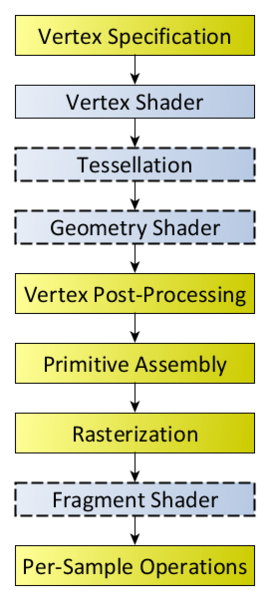
\includegraphics[scale=0.4]{imagens/openglPipeline.png}
	\caption{\small \textit{Rendering pipeline} OpenGL (Fonte: OpenGL, 2016)}
	\label{fig:glpipeline}
\end{figure}

O processo de execução de um programa que exibe resultados em um monitor gráfico requer uma série de etapas, com grande quantidade de cálculos (CLEMENTS, 2014). Assim como na CPU (\textit{Central Processing Unit}, Unidade de Processamento Central), que realiza o processamento geral do computador, a GPU (\textit{Graphics Processing Unit}, Unidade de Processamento Gráfico), também se beneficia de \textit{pipeline}.

Tal processo é definido pela execução paralela de múltiplas etapas, diminuindo a ociosidade do \textit{hardware} e aumentando a taxa de saída de dados (\textit{throuput}) (SHEN e LIPASTI, 2013). Logo que uma primeira instrução é finalizada em uma etapa, uma segunda pode iniciar, desde que não possua outras dependências.

A primeira etapa programável de processamento é o \textit{vertex shader}, sendo também a única obrigatória. Sua função é efetuar cálculos, tendo apenas um vértice como entrada e saída de dados (OpenGL, 2016b). Para funcionar corretamente, o programador deve especificar a entrada, chamada de \textit{vertex attribute}.

\begin{lstlisting}[language=glsl,
label={lst:vertexshader},
caption="Exemplo de \textit{vertex shader}"]
	#version 330
	layout (location = 0) in vec3 position;
	layout (location = 1) in vec3 normal;
	
	out vec3 Normal;
	out vec3 FragPos;
	
	uniform mat4 model;
	uniform mat4 view;
	uniform mat4 projection;
	
	void main()
	{
		gl_Position = projection * view *  model * vec4(position, 1.0f);
		FragPos = vec3(model * vec4(position, 1.0f));
		Normal = mat3(transpose(inverse(model))) * normal;  
	} 
}
\end{lstlisting}

No código \ref{lst:vertexshader}, podemos notar as entradas definidas por \lstinline{layout(location = #)} e as saídas por \lstinline{out}, que serão utilizadas na próxima etapa do \textit{pipeline}. Devido a natureza independente dos vértices, estes podem ser processados paralelamente em alta velocidade, fazendo uso dos múltiplos núcleos da GPU (AKENINE-MÖLLER et al, 2016).





%===================================================================================
%\backmatter
%===================================================================================

%\bibliography{monografia}{}
%\bibliographystyle{abnt-alf}

\begin{thebibliography}{9}

\bibitem{sage}MACHOVER, Carl. \textit{A Brief, Personal History of Computer Graphics}. 1978. p.38. Disponível em: \url{https://www.computer.org/csdl/mags/co/1978/11/01646756.pdf}.
Acesso em: 07 de junho de 2016.

\bibitem{toystory}GUHA, Sumanta. \textit{Computer Graphics Through OpenGL: From Theory to Experiments, Second Edition}. 2014. A K Peters/CRC Press. p.8-9.

\bibitem{irisgl}MARTZ, Paul. \textit{OpenGL Distilled}. 2016. Addison-Wesley Professional. p.26-8.

\bibitem{glbible}WRIGHT, Richard. HAEMEL, Nicholas. SELLERS, Graham. \textit{OpenGL SuperBible: Comprehensive Tutorial and Reference, 6th Edition}. 2013. Addison-Wesley Professional. p.4-9.

\bibitem{glsl1}ROST, Randi. LICEA-KANE, Bill. \textit{OpenGL Shading Language}. 2009. Addison-Wesley Professional. p.26-8.

%\bibitem{toystory}Pixar. 2016. \textit{Pixar Feature Films}. Disponível em: \url{http://www.pixar.com/features_films/TOY-STORY}.
%Acesso em: 08 de junho de 2016.

\bibitem{shaders}BAILEY, Mike. CUNNINGHAM, Steve. \textit{Graphic Shaders: Theory and Practice, 2nd Edition}. 2012. CRC Press. p.20-1.

\bibitem{glsl2}OpenGL. 2016. \textit{OpenGL Shading Language Specification}. Disponível em: \url{https://www.opengl.org/documentation/glsl/}.
Acesso em: 13 de junho de 2016.

\bibitem{gl2khronos}Khronos Group. 2016. \textit{OpenGL ARB to Pass Control of OpenGL Specification to Khronos Group}. Disponível em: \url{https://www.khronos.org/news/press/opengl_arb_to_pass_control_of_opengl_specification_to_khronos_group}.
Acesso em: 13 de junho de 2016.

\bibitem{glhistory}OpenGL. 2016a. \textit{History of OpenGL}. Disponível em: \url{https://www.opengl.org/wiki/History_of_OpenGL#Deprecation_Model}.
Acesso em: 15 de julho de 2016.

\bibitem{glsl2}Khronos Group. 2016. \textit{About The Khronos Group}. Disponível em: \url{https://www.khronos.org/about/}.
Acesso em: 13 de junho de 2016.

% --------------------------------------------------------------------

\bibitem{pipeline}CLEMENTS, Alan. \textit{Computer Organization \& Architecture: Themes and Variations}. 2014. Cengage Learning. p.858-861.

\bibitem{gpupipeline}SHEN, John. LIPASTI, Mikko. \textit{Modern Processor Design: Fundamentals of Superscalar Processors}. 2013. Waveland Press, Inc. p.40, 51.

\bibitem{renderpipeline}OpenGL. 2016b. \textit{Rendering Pipeline Overview}. Disponível em: \url{https://www.opengl.org/wiki/Rendering_Pipeline_Overview}.
Acesso em: 18 de julho de 2016.

\bibitem{openglspec}OpenGL. 2016c. \textit{The OpenGL Graphics System:
A Specification}. Disponível em: \url{https://www.opengl.org/registry/doc/glspec45.core.pdf}.
Acesso em: 19 de julho de 2016.

\bibitem{realtime}AKENINE-MÖLLER, Tomas. HAINES, Eric. HOFFMAN, Naty. \textit{Real-Time Rendering, Third Edition}. 2016. CRC Press. p.??????????.


\end{thebibliography}


\anexo
\end{document}